\chapter{Experimentos}
\thispagestyle{empty}

\section{Entornos}

\subsection{Entorno de desarrollo}
% En este apartado describimos el entorno que vamos a usar para entrenar el modelo.

El proyecto se llevó a cabo utilizando exclusivamente el lenguaje de programación \textit{Python}, debido a su versatilidad y eficacia en diversas áreas, desde el renderizado de modelos 3D en \textit{Blender} hasta el desarrollo de modelos de aprendizaje profundo. Se emplearon diversas bibliotecas para diferentes tareas: \textit{Trimesh} y \textit{PyVista} junto con \textit{VTK} para la manipulación de modelos 3D; \textit{Mediapipe} para la extracción de puntos de referencia faciales; \textit{NumPy} y \textit{pandas} para el procesamiento de datos; \textit{PIL} para el trabajo con imágenes; \textit{matplotlib} y \textit{Seaborn} para la generación de gráficos; \textit{Optuna} para la optimización de hiperparámetros; \textit{MLflow} para la gestión de experimentos; y, finalmente, \textit{PyTorch} junto con las librerías CUDA para el entrenamiento de modelos de aprendizaje profundo.

Con el objetivo de realizar un control de versiones durante el desarrollo del proyecto, se utilizó Git junto con GitHub. El código generado se puede encontrar en el siguiente enlace \url{https://github.com/ivansalinasugr/TFG}. Para más información, consultar el Readme del repositorio.

\subsection{Entorno de ejecución}

El proceso de ejecución se lleva a cabo en un entorno de alto rendimiento ubicado en la Universidad de Granada, al que se accede de forma remota a través de SSH. Se emplea un script de Shell para configurar los parámetros esenciales de los archivos. Por un lado, se utiliza SLURM para reservar recursos en la partición \enquote*{dios} del clúster, asignando una GPU del nodo \enquote*{dionisio}. Este nodo cuenta con dos Quadro RTX 8000, una memoria RAM de 512 GB DDR4 y dos procesadores Intel Xeon Silver 4216. Por otro lado, Conda se encarga de gestionar el entorno de software, garantizando la disponibilidad de las bibliotecas necesarias durante el proceso.

\section{Resultados}

[Esta parte está verde todavía porque estoy a la espera de que finalice la optimización de hiperparámetros y después el entrenamiento final de los modelos. Además, aunque la hice al principio, quiero hacer otra vez la comparativas de tiempos de Pytorch vs Keras.]

\subsection{Tiempos PyTorch vs Keras}


\subsection{Experimentos VGG-16}

Inicialmente, se llevó a cabo una fase de ajuste de hiperparámetros con el fin de determinar una configuración óptima para la arquitectura propuesta. Los rangos de valores y los parámetros finales se detallan en la Tabla \ref{hiper-vgg}. Además de los hiperparámetros mencionados, se estableció un entrenamiento a lo largo de 300 épocas, con una tasa de aprendizaje mínima de $10^{-12}$ y una reducción de la tasa de aprendizaje del 20\% cada 3 épocas consecutivas sin mejoras (paciencia), hasta un mínimo de $10^{-12}$.

\begin{table}[h]
	\centering
	\begin{tabular}{lll}
	\hline
	Parámetros          & Opciones                 & Mejor \\ \hline
	Optimizador         & {[}adam, sgd{]}          & adam  \\
	Tasa de aprendizaje & {[}$10^{-6}$, $10^{-3}${]}         & $4.63 \cdot 10^{-5}$      \\
	Tamaño del lote    & {[}16, 32, 64, 128{]}    & 32      \\
	Paciencia           & {[}2, 3, 4{]}            & 3     \\
	\textit{Early Stopping}     & {[}4, 6, 8{]}            & 6     \\
	\textit{Dropout} (\%)    & {[}0, 10, 20, 30{]} &  0 \\ \hline
	\end{tabular}
	\caption{Parámetros de entrenamiento seleccionados para la red VGG-16, junto a los rangos de valores utilizados durante el proceso de optimización de hiperparámetros.}
	\label{hiper-vgg}
\end{table}

A continuación, la Figura \ref{fig30} muestra la gráfica de la función de pérdida durante el entrenamiento, mientras que la Tabla \ref{met-ent-vgg16} muestra los valores finales de las métricas.

\begin{figure}[h]
	\centering
	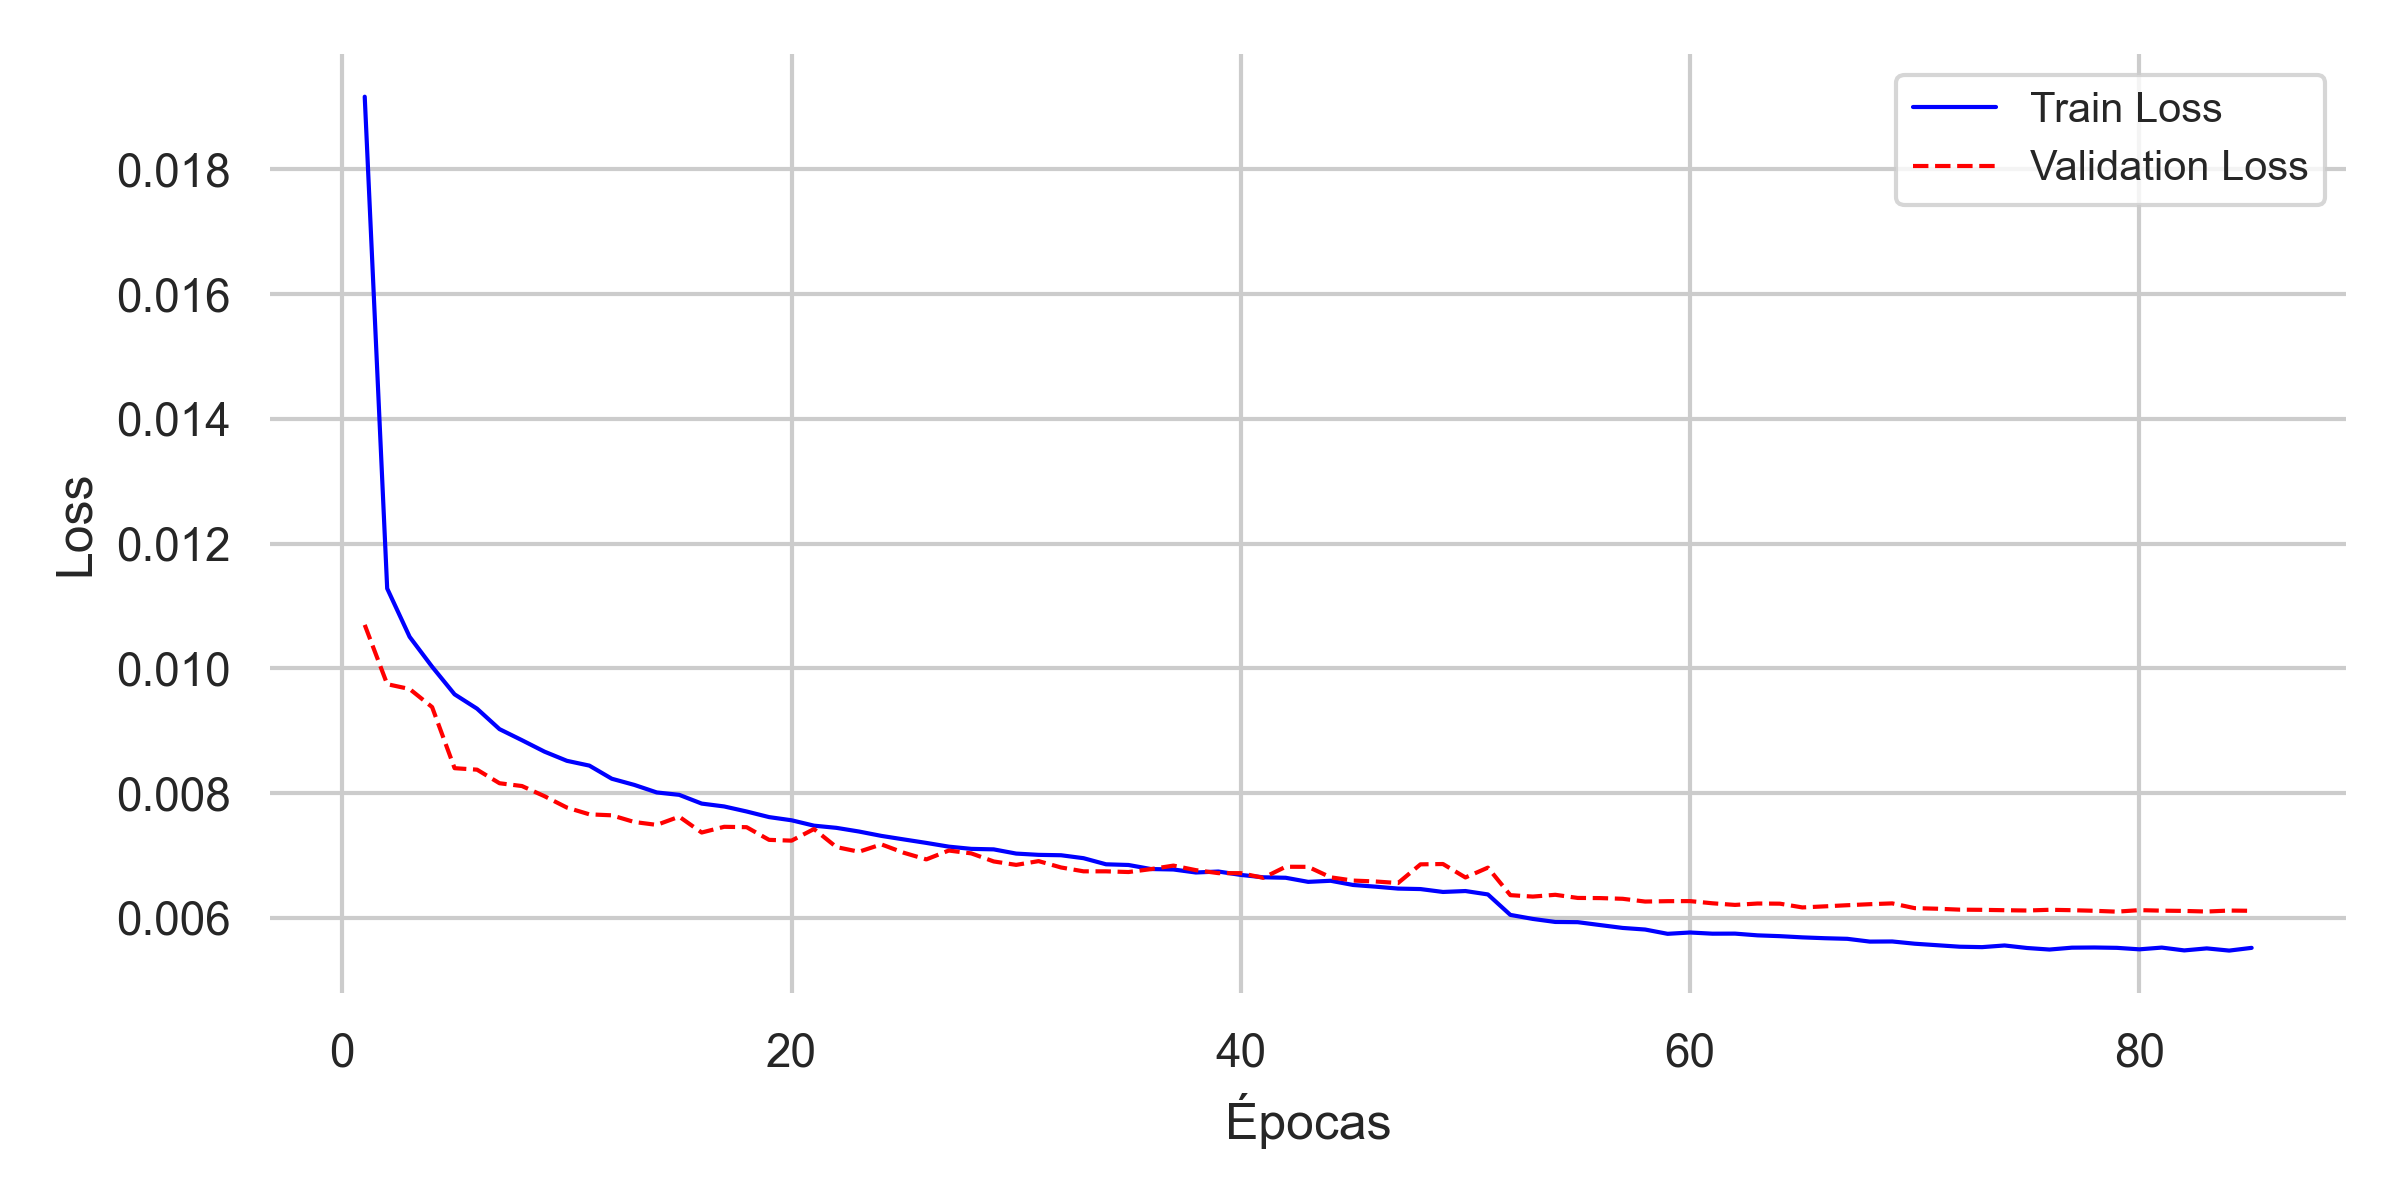
\includegraphics[scale=0.6]{imagenes/cap5/train_loss_vgg16.png}
	\caption[Gráfica de pérdida VGG-16.]{Gráfica de la función de pérdida durante el entrenamiento de la red VGG-16. En azul se representa la pérdida en el conjunto de entrenamiento mientras que en naranja se representa la pérdida en el conjunto de validación.}
	\label{fig30}
\end{figure}

\textbf{AQUÍ DISCUSIÓN RESULTADOS GRÁFICA}

\begin{table}[h]
	\centering
	\resizebox{\textwidth}{!}{%
	\begin{tabular}{llll}
	\hline
	Métricas de evaluación &
	   &
	  Entrenamiento &
	  Validación \\ \hline
	Distorsión &
	  \begin{tabular}[c]{@{}l@{}}Media (std)\\ Mediana\\ Mínimo\\ Perc 90, 95, 99\end{tabular} &
	  \begin{tabular}[c]{@{}l@{}}0.005 (0.004)\\ 0.003\\ 0.0\\ {[}0.01, 0.013, 0.02{]}\end{tabular} &
	  \begin{tabular}[c]{@{}l@{}}0.006 (0.006)\\ 0.004\\ 0.0\\ {[}0.014, 0.017, 0.027{]}\end{tabular} \\ \hline
	MAE (cm) &
	  \begin{tabular}[c]{@{}l@{}}Media (std)\\ Mediana\\ Mínimo\\ Perc 90, 95, 99\end{tabular} &
	  \begin{tabular}[c]{@{}l@{}}24.696 (35.699)\\ 9.258\\ 0.0\\ {[}70.687, 100.423, 164.784{]}\end{tabular} &
	  \begin{tabular}[c]{@{}l@{}}31.425 (44.048)\\ 12.194\\ 0.0\\ {[}89.95, 125.105, 204.385{]}\end{tabular} \\ \hline
	MRE (\%) &
	  \begin{tabular}[c]{@{}l@{}}Media (std)\\ Mediana\\ Mínimo\\ Perc 90, 95, 99\end{tabular} &
	  \begin{tabular}[c]{@{}l@{}}0.085 (0.103)\\ 0.057\\ 0.0\\ {[}0.183, 0.254, 0.487{]}\end{tabular} &
	  \begin{tabular}[c]{@{}l@{}}0.111 (0.138)\\ 0.075\\ 0.0\\ {[}0.233, 0.328, 0.647{]}\end{tabular} \\ \hline
	\end{tabular}%
	}
	\caption{Métricas en los conjuntos de entrenamiento y de validación tras el proceso de entrenamiento de la red VGG-16.}
	\label{met-ent-vgg16}
\end{table}

\textbf{AQUÍ DISCUSIÓN RESULTADOS MÉTRICAS}

\subsection{Experimentos ResNet-50}

Al igual que con VGG-16, primero se llevó a cabo una fase de ajuste de hiperparámetros con el fin de determinar una configuración óptima para la arquitectura propuesta. Los rangos de valores y los parámetros finales se detallan en la Tabla \ref{hiper-resnet}. Además de los hiperparámetros mencionados, se estableció un entrenamiento a lo largo de 300 épocas, con una tasa de aprendizaje mínima de $10^{-12}$ y una reducción de la tasa de aprendizaje del 20\% cada 3 épocas consecutivas sin mejoras (paciencia), hasta un mínimo de $10^{-12}$.

\begin{table}[h]
	\centering
	\begin{tabular}{lll}
	\hline
	Parámetros          & Opciones                 & Mejor \\ \hline
	Optimizador         & {[}adam, sgd{]}          &   \\
	Tasa de aprendizaje & {[}$10^{-6}$, $10^{-3}${]}         &       \\
	Tamaño del lote     & {[}16, 32, 64, 128{]}    &       \\
	Paciencia           & {[}2, 3, 4{]}            &      \\
	Parada temprana     & {[}4, 6, 8{]}            &      \\
	\textit{Dropout} (\%)    & {[}0, 10, 20, 30{]} &    \\ \hline
	\end{tabular}
	\caption{Parámetros de entrenamiento seleccionados para la red ResNet-50, junto a los rangos de valores utilizados durante el proceso de optimización de hiperparámetros.}
	\label{hiper-resnet}
\end{table}

A continuación, la Figura X muestra la gráfica de la función de pérdida durante el entrenamiento, mientras que la Tabla \ref{met-ent-resnet} muestra los valores finales de las métricas.

Figura X

\begin{table}[h]
	\centering
	\begin{tabular}{lll}
	\hline
	Métricas de evaluación &                                                                                          & Valor \\ \hline
	Distorsión & \begin{tabular}[c]{@{}l@{}}Media (std)\\ Mediana\\ Mínimo\\ Perc 90, 95, 99\end{tabular} &  \\ \hline
	MAE (cm)               & \begin{tabular}[c]{@{}l@{}}Media (std)\\ Mediana\\ Mínimo\\ Perc 90, 95, 99\end{tabular} &       \\ \hline
	MRE (\%)               & \begin{tabular}[c]{@{}l@{}}Media (std)\\ Mediana\\ Mínimo\\ Perc 90, 95, 99\end{tabular} &       \\ \hline
	\end{tabular}
	\caption{Métricas en los conjuntos de entrenamiento y de validación tras el proceso de entrenamiento de la red ResNet-50.}
	\label{met-ent-resnet}
\end{table}

Aquí discusión sobre los resultados.


\subsection{Comparación FSCDnet}

Aquí se haría una comparativa de los dos modelos de FacialSCDnet+ contra los modelos tanto sintéticos como reales entrenados en FSCDnet. Habría dos comparativas, una con los datos de test de FSCDnet (que son fotografías reales), y otra con los datos de test de FSCDnet+ (conjunto de test con algunos sujetos que se reservaron completamente). Se pondría tanto una tabla comparando las métricas, como los diagramas de caja y de violín, junto con una gráfica de comparación entre etiquetas predichas y verdaderas.


\begin{table}[h]
	\centering
	\resizebox{\textwidth}{!}{%
	\begin{tabular}{llllll}
	\hline
	\begin{tabular}[c]{@{}l@{}}Métricas de \\ evaluación\end{tabular} &
	   &
	  \begin{tabular}[c]{@{}l@{}}VGG-16 \\ FSCDnet+\end{tabular} &
	  \begin{tabular}[c]{@{}l@{}}ResNet-50 \\ FSCDnet+\end{tabular} &
	  \begin{tabular}[c]{@{}l@{}}VGG-16 \\ FSCDnet real\end{tabular} &
	  \begin{tabular}[c]{@{}l@{}}VGG-16 \\ FSCDnet synth\end{tabular} \\ \hline
	Distorsión & \begin{tabular}[c]{@{}l@{}}Media (std)\\ Mediana\\ Mínimo\\ Perc 90, 95, 99\end{tabular} &  &  &  &  \\ \hline
	MAE (cm)   & \begin{tabular}[c]{@{}l@{}}Media (std)\\ Mediana\\ Mínimo\\ Perc 90, 95, 99\end{tabular} &  &  &  &  \\ \hline
	MRE (\%)   & \begin{tabular}[c]{@{}l@{}}Media (std)\\ Mediana\\ Mínimo\\ Perc 90, 95, 99\end{tabular} &  &  &  &  \\ \hline
	\end{tabular}%
	}
	\caption{Métricas en el conjunto de test de FacialSCDnet+, comparando los modelos VGG-16 y ResNet-50 de FacialSCDnet+ contra los modelos real y sintético de FacialSCDnet.}
	\label{test-mio}
\end{table}

\begin{table}[h]
	\centering
	\resizebox{\columnwidth}{!}{%
	\begin{tabular}{llllll}
	\hline
	\begin{tabular}[c]{@{}l@{}}Métricas de \\ evaluación\end{tabular} &
	   &
	  \begin{tabular}[c]{@{}l@{}}VGG-16 \\ FSCDnet+\end{tabular} &
	  \begin{tabular}[c]{@{}l@{}}ResNet-50 \\ FSCDnet+\end{tabular} &
	  \begin{tabular}[c]{@{}l@{}}VGG-16 \\ FSCDnet real\end{tabular} &
	  \begin{tabular}[c]{@{}l@{}}VGG-16 \\ FSCDnet synth\end{tabular} \\ \hline
	Distorsión & \begin{tabular}[c]{@{}l@{}}Media (std)\\ Mediana\\ Mínimo\\ Perc 90, 95, 99\end{tabular} &  &  &  &  \\ \hline
	MAE (cm)   & \begin{tabular}[c]{@{}l@{}}Media (std)\\ Mediana\\ Mínimo\\ Perc 90, 95, 99\end{tabular} &  &  &  &  \\ \hline
	MRE (\%)   & \begin{tabular}[c]{@{}l@{}}Media (std)\\ Mediana\\ Mínimo\\ Perc 90, 95, 99\end{tabular} &  &  &  &  \\ \hline
	\end{tabular}%
	}
	\caption{Métricas en el conjunto de test real de FacialSCDnet, comparando los modelos VGG-16 y ResNet-50 de FacialSCDnet+ contra los modelos real y sintético de FacialSCDnet.}
	\label{test}
\end{table}

Aquí la discusión de los resultados.